%% \documentclass[landscape,final,a0paper,fontscale=0.285]{baposter}
%% \documentclass[landscape,final,a0paper,fontscale=0.4]{baposter}
\documentclass[landscape,final,a0paper,fontscale=0.35]{baposter}

\usepackage{calc}
\usepackage{graphicx}
\usepackage{amsmath}
\usepackage{amssymb}
\usepackage{relsize}
\usepackage{multirow}
\usepackage{rotating}
\usepackage{bm}
\usepackage{url}

\usepackage{graphicx}
\usepackage{multicol}

%% \usepackage{times}
%% \usepackage{helvet}
%\usepackage{bookman}
\usepackage{palatino}

\usepackage{lipsum}
%% \usepackage{jabbrv}
%% \usepackage{setspace}
\usepackage{enumitem}

\newcommand{\captionfont}{\footnotesize}

\graphicspath{{../paper/figures/}}
%% \graphicspath{{images/}{../images/}}
%% \usetikzlibrary{calc}

%%%%%%%%%%%%%%%%%%%%%%%%%%%%%%%%%%%%%%%%%%%%%%%%%%%%%%%%%%%%%%%%%%%%%%%%%%%%%%%%
%%%% Some math symbols used in the text
%%%%%%%%%%%%%%%%%%%%%%%%%%%%%%%%%%%%%%%%%%%%%%%%%%%%%%%%%%%%%%%%%%%%%%%%%%%%%%%%

%%%%%%%%%%%%%%%%%%%%%%%%%%%%%%%%%%%%%%%%%%%%%%%%%%%%%%%%%%%%%%%%%%%%%%%%%%%%%%%%
% Multicol Settings
%%%%%%%%%%%%%%%%%%%%%%%%%%%%%%%%%%%%%%%%%%%%%%%%%%%%%%%%%%%%%%%%%%%%%%%%%%%%%%%%
\setlength{\columnsep}{1.5em}
\setlength{\columnseprule}{0mm}

%%%%%%%%%%%%%%%%%%%%%%%%%%%%%%%%%%%%%%%%%%%%%%%%%%%%%%%%%%%%%%%%%%%%%%%%%%%%%%%%
% Save space in lists. Use this after the opening of the list
%%%%%%%%%%%%%%%%%%%%%%%%%%%%%%%%%%%%%%%%%%%%%%%%%%%%%%%%%%%%%%%%%%%%%%%%%%%%%%%%
\newcommand{\compresslist}{%
\setlength{\itemsep}{1pt}%
\setlength{\parskip}{0pt}%
\setlength{\parsep}{0pt}%
}

%%%%%%%%%%%%%%%%%%%%%%%%%%%%%%%%%%%%%%%%%%%%%%%%%%%%%%%%%%%%%%%%%%%%%%%%%%%%%%
%%% Begin of Document
%%%%%%%%%%%%%%%%%%%%%%%%%%%%%%%%%%%%%%%%%%%%%%%%%%%%%%%%%%%%%%%%%%%%%%%%%%%%%%

\begin{document}

%%%%%%%%%%%%%%%%%%%%%%%%%%%%%%%%%%%%%%%%%%%%%%%%%%%%%%%%%%%%%%%%%%%%%%%%%%%%%%
%%% Here starts the poster
%%%---------------------------------------------------------------------------
%%% Format it to your taste with the options
%%%%%%%%%%%%%%%%%%%%%%%%%%%%%%%%%%%%%%%%%%%%%%%%%%%%%%%%%%%%%%%%%%%%%%%%%%%%%%
% Define some colors

%\definecolor{lightblue}{cmyk}{0.83,0.24,0,0.12}
%% \definecolor{lightblue}{rgb}{0.145,0.6666,1}

%% \definecolor{headerfade}{rgb}{0.89,0.68,0}
\definecolor{headerfade}{rgb}{0.93, 0.80, 0.38}

\hyphenation{resolution occlusions}
%%
\begin{poster}%
  % Poster Options
  {
  % Show grid to help with alignment
  grid=false,
  columns=4,
  % Column spacing
  colspacing=1em,
  % Color style
  bgColorOne=white,
  bgColorTwo=white,
  borderColor=headerfade,
  headerColorOne=black,
  headerColorTwo=headerfade,
  headerFontColor=white,
  boxColorOne=white,
  boxColorTwo=headerfade,
  % Format of textbox
  textborder=roundedleft,
  % Format of text header
  eyecatcher=true,
  headerborder=closed,
  headerheight=0.17\textheight,
%  textfont=\sc, An example of changing the text font
  headershape=roundedright,
  headershade=shadelr,
  headerfont=\Large\bf\textsc, %Sans Serif
  textfont={\setlength{\parindent}{1.5em}},
  boxshade=plain,
%  background=shade-tb,
  background=plain,
  linewidth=2pt
  }
  % Eye Catcher
  {
    \begin{tabular}{c}
      \relax\\
      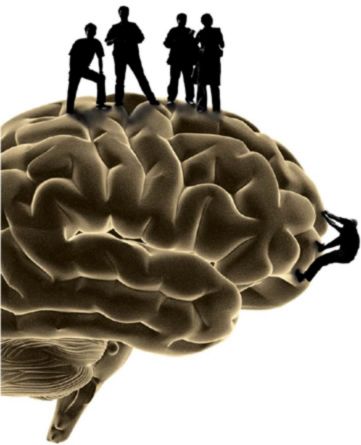
\includegraphics[height=13em]{brain.png}
    \end{tabular}
  }
  % Title
  {
    \textbf{\textsc{Selective Processing for Real-time Stereo Matching}}\vspace{0.5em}
  }
  % Authors
  {
    \textsc{Eric Hunsberger, Jeff Orchard, Bryan Tripp}\\[0.2em]
    \{ehunsber, jeff.orchard, bptripp\}@uwaterloo.ca\\[0.4em]
    %% Centre for Theoretical Neuroscience, University of Waterloo (\url{http://ctn.uwaterloo.ca})
  }
  % University logo
  {
    %% 
\includegraphics[height=9.0em]{ctn.png}
    \begin{tabular}{cc}
      \relax\\
      
\includegraphics[height=6.0em]{uwaterloo.png} &
      
\includegraphics[height=5.0em]{ctn.png}\\
      \multicolumn{2}{c}{
        
\includegraphics[height=5.0em]{cnrg.png}}
    \end{tabular}
  }

%%%%%%%%%%%%%%%%%%%%%%%%%%%%%%%%%%%%%%%%%%%%%%%%%%%%%%%%%%%%%%%%%%%%%%%%%%%%%%
%%% Now define the boxes that make up the poster
%%%---------------------------------------------------------------------------
%%% Each box has a name and can be placed absolutely or relatively.
%%% The only inconvenience is that you can only specify a relative position
%%% towards an already declared box. So if you have a box attached to the
%%% bottom, one to the top and a third one which should be in between, you
%%% have to specify the top and bottom boxes before you specify the middle
%%% box.
%%%%%%%%%%%%%%%%%%%%%%%%%%%%%%%%%%%%%%%%%%%%%%%%%%%%%%%%%%%%%%%%%%%%%%%%%%%%%%
    %
    % A coloured circle useful as a bullet with an adjustably strong filling
    \newcommand{\colouredcircle}{%
      \tikz{\useasboundingbox (-0.2em,-0.32em) rectangle(0.2em,0.32em); \draw[draw=black,fill=headerfade,line width=0.03em] (0,0) circle(0.18em);}}

    \newenvironment{blockitemize}
    {%
      \begin{minipage}{\columnwidth - 2em}
      \begin{itemize}
        \setlength{\itemsep}{0.3em}

        \raggedright
    }{
      \end{itemize}
      \end{minipage}
    }

    %%%%%%%%%%%%%%%%%%%%%%%%%%%%%%%%%%%%%%%%%%%%%%%%%%%%%%%%%%%%%%%%%%%%%%%%%%%%%%%%

    \headerbox{Introduction}{name=pane00,column=0,row=0}{
      \noindent
      TODO
    }

    \headerbox{Methods}{name=pane01,column=0,below=pane00}{
      TODO
      %% \begin{description}[noitemsep, nolistsep]
      %%   \newcommand{\dline}{\hfill\\}
      %%   \item[Input:] An aperiodic random signal\\(amplitude = 0.1, max. frequency = 5 Hz)
      %%   \item[Neurons:] 64 Fitzhugh-Nagumo (FHN)\\
      %%     or leaky integrate-and-fire (LIF) model neurons
      %%   \item[Noise:] Gaussian white noise added to neuron membrane
      %%   \item[Heterogeneity:]
      %%     Introduced by choosing neuron bias currents from uniform distributions
      %%     (larger distribution radius corresponds to increased heterogeneity)
      %%   \item[Output:] Summed and filtered spikes from all neurons
      %%   \item[Performance metric:] Mutual information calculated between input and output signals
      %% \end{description}

      %% %% \vspace{1em}
      %% \begin{center}
      %%   %% \includegraphics[width=\columnwidth]{../figures/experiment.pdf}
      %% \end{center}
    }

    \headerbox{References}{name=pane02,column=0,below=pane01,above=bottom}{
      %% \scriptsize
      %% \renewcommand{\refname}{\vspace{-0.8em}}
      %% \bibliographystyle{jabbrv_ieeetr}
      %% \bibliography{/media/dropbox/papers/bib/Publishing-StochasticResonance}
    }

    \headerbox{Fovea Example}{name=pane10,column=1,row=0}{
      \begin{center}
        %% \includegraphics[width=0.75\columnwidth, clip=true, trim=3mm 6mm 3mm 4mm]
        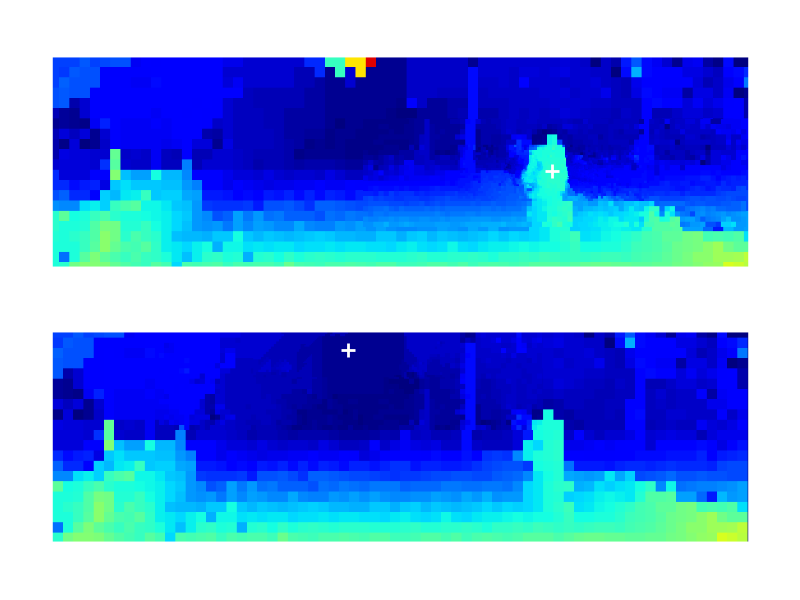
\includegraphics[width=1.0\columnwidth]{fovea-examples.png}
      \end{center}
    }

    \headerbox{Something}{name=pane11,column=1,row=0,below=pane10}{
      \begin{center}
        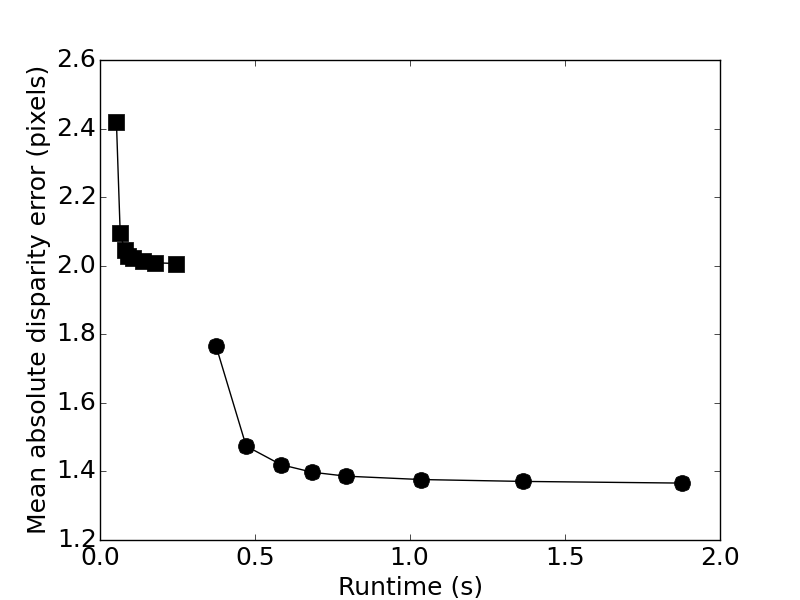
\includegraphics[width=1.0\columnwidth]{fovea-rationale.png}
      \end{center}
    }

    \headerbox{Importance}{name=pane20,column=2,row=0}{
      \begin{center}
        %% 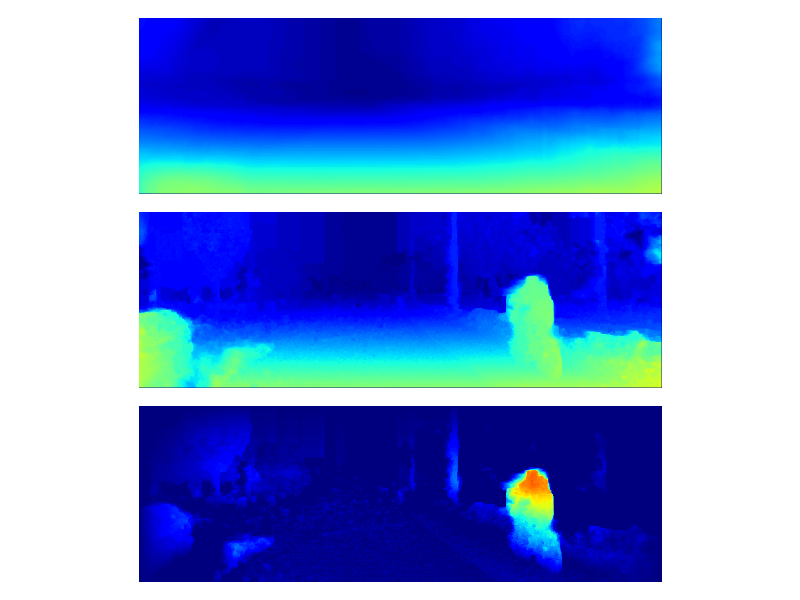
\includegraphics[width=1.0\columnwidth]{importance.png}
        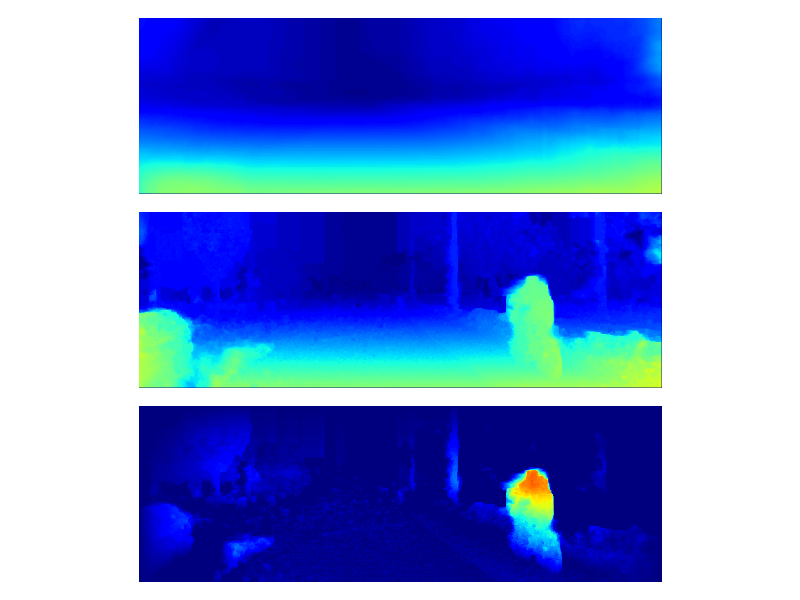
\includegraphics[width=1.0\columnwidth,clip=true,trim=30mm 0mm 30mm 0mm]{importance.png}
      \end{center}
    }

    \headerbox{Foveation sequence}{name=pane21,column=2,row=0,below=pane20}{
      TODO
      \begin{center}
        %% 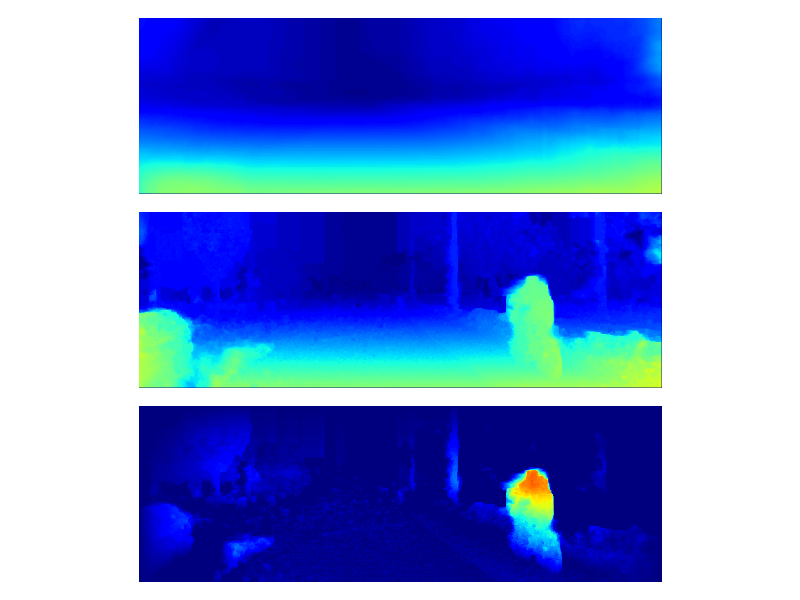
\includegraphics[width=1.0\columnwidth]{importance.png}
      \end{center}
    }

    \headerbox{Something}{name=pane30,column=3,row=0}{
    }

    \headerbox{Conclusions}{name=pane31,column=3,row=0,below=pane30}{
      \noindent
      \begin{blockitemize}
        \item TODO
        %% \item Computing the fine data cost and downsampling has
      \end{blockitemize}
    }

    \headerbox{Future Work}{name=pane32,column=3,row=0,below=pane31}{
      \noindent
      \begin{blockitemize}
        \item Use coarser resolution outside fovea to further reduce computation
        \item Use multiple foveas to target multiple regions of interest
      \end{blockitemize}
    }


    %% \headerbox{Resonance and Heterogeneity}{name=reshetero,column=1,row=0}{
    %%   %% \noindent
    %%   %% Both heterogeneity and noise can help populations encode signals, in the right amounts.
    %%   %% In the figure below, we see resonance with respect to heterogeneity:
    %%   \begin{center}
    %%     %% \includegraphics[width=0.75\columnwidth, clip=true, trim=3mm 6mm 3mm 4mm]
    %%     %%                 {../figures/color/infohetero.pdf}
    %%   \end{center}
    %% }
    %% \headerbox{Resonance and Noise}{name=resnoise,column=1,below=reshetero}{
    %%   \begin{center}
    %%     %% \includegraphics[width=\columnwidth, clip=true, trim=3mm 6mm 3mm 4mm]
    %%     %%                 {../figures/color/info.pdf}
    %%   \end{center}

    %%   \noindent
    %%   \begin{blockitemize}
    %%     \item LIF neurons exhibit resonance only at low levels of heterogeneity
    %%     \item FHN neurons exhibit resonance at all levels of heterogeneity,
    %%       since heterogeneity cannot fully desynchronize neurons
    %%   \end{blockitemize}
    %% }

    %% \headerbox{Redundant Benefits}{name=body,column=1,span=2,below=resnoise,above=bottom}{
    %%   \begin{multicols}{2}
    %%     \noindent
    %%     Since heterogeneity and noise operate through similar mechanisms,
    %%     their benefits are not additive.

    %%     \noindent
    %%     \begin{blockitemize}
    %%       \vspace{0.5em}
    %%       \item For LIF neurons (right), overall information encoding is optimized for
    %%         biases chosen from the range $b_i \in [-0.15, 0.15]$ and no noise
    %%       \item Given optimal heterogeneity,
    %%         adding noise ($\sigma_\eta~=~10^{-2}$) reduces encoded information
    %%       \item But in the absence of heterogeneity,
    %%         a moderate amount of noise ($\sigma_\eta = 10^{-2}$) optimizes encoded information
    %%         (see \textsc{Resonance and Noise})
    %%     \end{blockitemize}

    %%     \begin{center}
    %%       %% \includegraphics[width=0.78\columnwidth]{../figures/color/infocontour.pdf}
    %%     \end{center}
    %%   \end{multicols}
    %% }

    %% \headerbox{Desynchronization}{name=desynchronization,column=2,above=body}{
    %%   \noindent
    %%   \raggedright
    %%   Noise~\cite{Stocks2001a} and heterogeneity~\cite{Burton2012}
    %%   desynchronize neuronal spiking.
    %%   %% We quantified these results %in our experiments
    %%   %% by measuring the standard deviation of the phase across a population of neurons,
    %%   %% and varying the level of noise and heterogeneity in the population.

    %%   \noindent
    %%   \begin{blockitemize}
    %%     \vspace{0.5em}
    %%     \item FHN neurons have about the same firing rate for all stimuli above the firing threshold,
    %%       so heterogeneity in the biases is not able to fully desynchronize them
    %%     \item In LIF neurons, heterogeneity is slightly better than noise at desynchronizing neuronal firing
    %%   \end{blockitemize}

    %%   \begin{center}
    %%     %% \includegraphics[width=\columnwidth, clip=true, trim=3mm 6mm 3mm 4mm]
    %%     %%                 {../figures/color/phase.pdf}
    %%   \end{center}

    %%   \noindent
    %%   \begin{center}
    %%   \begin{minipage}{0.33\columnwidth}
    %%     \raggedright
    %%     Spike rasters for LIF neurons
    %%     with low noise (top) and high noise (bottom)
    %%     demonstrate that noise reduces synchrony.
    %%     %% The nois neurons fire more asynchronously.
    %%   \end{minipage}
    %%   \begin{minipage}{0.63\columnwidth}
    %%     \vspace{-1em}
    %%     \begin{center}
    %%       %% \includegraphics[width=1.05\columnwidth, clip=true, trim=1mm 3mm 1mm 1mm]
    %%       %%                 {../figures/color/syncraster.pdf}
    %%     \end{center}
    %%   \end{minipage}
    %%   \end{center}
    %% }

    %% \headerbox{Linearization}{name=linearization,column=3}{
    %%   \raggedright
    %%   \noindent
    %%   Noise can improve population encoding by linearizing neuron stimulus-response curves~\cite{Chance2002}:
    %%   \begin{center}
    %%     %% \includegraphics[width=\columnwidth, clip=true, trim=3mm 6mm 3mm 4mm]
    %%     %%                 {../figures/color/tuningnoisy.pdf}
    %%   \end{center}

    %%   \noindent
    %%   Heterogeneity linearizes the \emph{population} stimulus-response:
    %%   %% as illustrated below.
    %%   %% The population tuning curves (left) are averaged to form the population response (right, black line),
    %%   %% which is more linear than a homogeneous population response (right, dashed line).
    %%   \begin{center}
    %%     %% \includegraphics[width=\columnwidth, clip=true, trim=3mm 4mm 3mm 4mm]
    %%     %%                 {../figures/color/tuninghetero.pdf}
    %%   \end{center}

    %% }

    %% \headerbox{Future work}{name=future,column=3,above=bottom}{
    %%   \noindent
    %%   \begin{blockitemize}
    %%     \item Examine more sophisticated neuron models and other decoding methods
    %%     \item Extend heterogeneity to other neuron parameters
    %%       (\emph{e.g.,} maximum firing rate)
    %%       to determine if this increases the benefits of heterogeneity in FHN neurons
    %%     \item Quantify these effects
    %%       in the context of a functional multi-layer model of the visual system
    %%   \end{blockitemize}
    %% }

    %% \headerbox{Conclusions}{name=conclusions,column=3,above=future,below=linearization}{
    %%   \noindent
    %%   \begin{blockitemize}
    %%     \raggedright
    %%     \item Noise and heterogeneity both provide a neuronal population
    %%       with a better basis for encoding signals
    %%     \item This is done by desynchronizing neuronal firing and linearizing neuron tuning curves
    %%     \item Both noise and heterogeneity show resonance effects,
    %%       offering increases in information encoding only across finite ranges
    %%     \item The benefits of noise and heterogeneity are not additive;
    %%       only one or the other is required
    %%   \end{blockitemize}

    %% }

\end{poster}
\end{document}

%%  LocalWords:  headerfade rgb colspacing bgColorOne bgColorTwo FHN
%%  LocalWords:  borderColor headerColorOne headerColorTwo textborder
%%  LocalWords:  headerFontColor boxColorOne boxColorTwo roundedleft
%%  LocalWords:  eyecatcher headerborder headerheight headershape LIF
%%  LocalWords:  roundedright headershade shadelr headerfont textfont
%%  LocalWords:  boxshade linewidth Eliasmith ehunsber mscott Nagumo
%%  LocalWords:  celiasmith uwaterloo Fitzhugh reshetero resnoise
%%  LocalWords:  rasters multi
